%!tex engine=xelatex
\documentclass[a4paper]{article}

\usepackage[margin=1.5in]{geometry}
\usepackage{amsmath,amssymb}
\usepackage{aastexmacros}
\usepackage{graphicx}
\usepackage{hyperref}

\usepackage{natbib}
\bibliographystyle{unsrtnat}

\usepackage{fontspec}
\setmainfont{EB Garamond}

\newcommand{\defn}[1]{\emph{#1}}

\title{Measuring Faraday Complexity}
\author{Matthew J. Alger\\{\small Research School of Astronomy and Astrophysics, ANU}\\{\small Data61, CSIRO}}

\begin{document}
    \maketitle

    \section{The Faraday Effect}

    The \defn{Faraday effect} is the rotation of light as it passes through a magnetic field. The amount of rotation is wavelength-dependent. This rotation and its variation over wavelengths can be measured with radio telescopes, giving us insight into physical processes between the source and the observer.

    Linear polarisation $P$ can be decomposed as the Stokes $I$, $Q$ and $U$ parameters following \citet{burn66depolarization} and \citet{bell12faraday}:
    \[
        P(\lambda) = Q(\lambda) + iU(\lambda) = \int_{-\infty}^{\infty} e^{2i\phi\lambda^2} F(\phi)\ d\phi.
    \]
    $\phi$ is the \defn{Faraday depth}, measured in $\mathrm{rad}\ \mathrm{m}^{-2}$. This is interpretable as a measure of how much rotation an intervening medium gives to an intrinsic polarisation angle as a linear function of $\lambda^2$. Note that this looks a lot like a Fourier transform of $F(\phi)$, which we call the \defn{Faraday spectrum}. For a simple source with rotation at just one Faraday depth $\phi_0$, $F(\phi) = \delta(\phi - \phi_0)$ and
    \begin{align*}
        P(\lambda) &= pI \int_{-\infty}^{\infty} e^{2i\phi\lambda^2} \delta(\phi - \phi_0)\ d\phi\\
            &= pI e^{2i\phi_0\lambda^2}\\
            &= pI \cos (2\phi_0\lambda^2) + i pI \sin (2\phi_0\lambda^2).
    \end{align*}
    We can then identify $Q = pI \cos(2 \phi_0 \lambda^2), U = pI \sin(2 \phi_0 \lambda^2)$ and hence the polarisation angle $\chi$ can be written
    \[
        \frac{1}{2} \mathrm{arctan}\ \frac{U}{Q} = \phi_0 \lambda^2,
    \]
    i.e. $\phi_0$ is the gradient of the polarisation angle as a function of $\lambda^2$. This relationship holds more generally for a quantity called the \defn{rotation measure} $RM$ which is equal to $\phi_0$ only for this simple case:
    \[
        RM = \frac{\partial \chi}{\partial \lambda^2}.
    \]

    We can write the Faraday depth of the point $r$ (with respect to an observer at $r = 0$) in physical terms $\phi(r)$ is the \defn{Faraday depth} of the point $r$ (with respect to an observer at $r = 0$). The Faraday depth carries physical meaning, with
    \[
        \phi(r) = \frac{e^3}{2\pi m_e^2 c^4} \int_0^r n_e(l) B_{||}(l)\ dl.
    \]
    $n_e$ is the electron density and $B_{||}$ is the line-of-sight magnetic field strength. $\phi$ is measured in $\mathrm{rad}\ \mathrm{m}^{-2}$.

    \begin{figure}
        \centering
        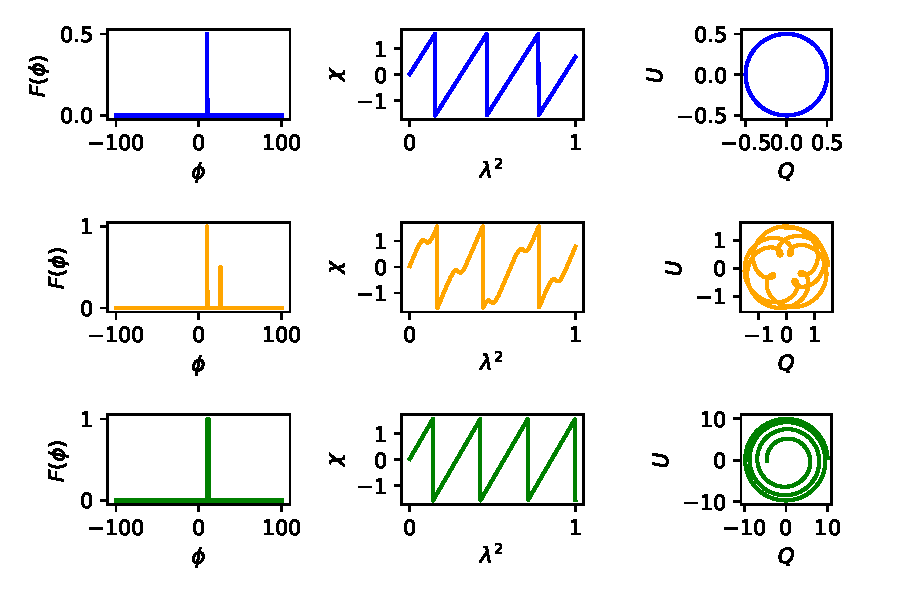
\includegraphics[width=0.8\textwidth]{faraday-depth.pdf}
        \caption{Different Faraday depth distributions (left) lead to different polarisation spectra (centre) and different-shaped $Q$/$U$ plots (right). Here we show a Faraday screen (top), two Faraday screens (centre), and a Faraday slab (bottom). \label{fig:faraday-depth-models}}
    \end{figure}

    More complex models are commonly applied. These are usually combinations of tophat and delta functions. Some of these models are shown in \autoref{fig:faraday-depth-models}.

    \section{Faraday Complexity}

    \defn{Faraday complexity} is a measure of how complex a polarised Faraday spectrum is. It's unclear exactly what a good Faraday complexity metric would look like, but at minimum a spectrum can be \defn{Faraday simple} if it is well-fit by a single Faraday screen. A spectrum that is not Faraday simple is then \defn{Faraday complex}. Perhaps we could even have some kind of `score', where higher numbers indicate `more' Faraday complexity.

    A brief summary of Faraday complexity classification methods can be found in Section 4.5 of \citet{anderson15faraday}. Another summary can be found in POSSUM Report \#68 \citep{purcell17complexity}. Methods include
    \begin{enumerate}
        \item nonlinearity of $\chi(\lambda^2)$ \citep{goldstein84-3c27},
        \item frequency-dependent change in $p$ \citep{farnes14catalogue},
        \item non-sinusoidal variation in $q$ and $u$ \citep{osullivan12agn},
        \item detection of multiple Faraday depth components after deconvolution \citep{law11spectropolarimetry},
        \item the second moment of the Faraday spectrum \citep{brown11report09},
        \item a convolutional neural network trained on simulated sources \citep{brown19classification}.
    \end{enumerate}
    There are problems with each of these approaches:
    \begin{enumerate}
        \item $\chi(\lambda^2)$ can be linear even for Faraday complex sources,
        \item $p$ is biased in hard-to-debias ways,
        \item works best (only?) for Faraday thin sources,
        \item requires deconvolution (itself an error-prone and complicated process),
        \item has many false negatives (but no false positives),
        \item works only for two-screen models and has been tested only on simulated data.
    \end{enumerate}

    \section{Complexity in POSSUM}

    One open question is ``how often are sources Faraday complex?''. \citet{anderson16faraday} suggest that with sufficiently dense frequency sampling \emph{almost all} sources are Faraday complex. At lower sampling density they find about half of their sources are Faraday complex. We have little idea how common Faraday complex sources are in general (and this is compounded by the lack of good definition of `Faraday complex'). An estimation of upper and lower complexity rates in POSSUM would be extremely valuable to the survey as well as future polarisation studies.

    It also remains an open question as to how much influence the Galactic magnetic field has on Faraday complexity of extragalactic sources. The Galactic magnetic field should induce a co-dependency between nearby sources, i.e. the polarisation spectrum of neighbouring sources isn't independent. Anywhere there is additional Faraday rotation besides the Galaxy we should observe Faraday complexity in its simplest definition (as non-Faraday simple). Questions in this domain include
    \begin{itemize}
        \item Can we explicitly account for/model the Galactic magnetic field, either for eliminating it or learning its structure?
        \item Can we utilise the dependencies in neighbouring sources to improve our model fits and complexity estimates?
        \item Can we define a Faraday complexity measure that excludes the Galactic magnetic field?
    \end{itemize}

    \bibliography{faraday-complexity}


\end{document}